\documentclass[../HFT-main.tex]{subfiles}
\begin{document}
\title{Contextual Framework for  Open Atomic Ethernet}

%\section{Æthernet Design Philosophy}
\section{Introduction}

It would be a mistake to assume conventional network concepts and terminology that you already know and love will remain unscathed in this project. While we have no intention of reinventing the wheel, yet some new concepts and terminology will be necessary in order to escape the quagmire of incrementalism of the last five decades. %in Networking. %, which has plagued the networking world for five decades. Old Concepts to unlearn:

\marginnote{We carefully described in four presentations why the concept of time is widely misunderstood in the OCP TAP (Time Appliance Community).  We respectfully request that you watch those presentations before insisting on timestamps or synchronized time in the context of Open Atomic Ethernet. \href{https://www.opencompute.org/w/index.php?title=Open_Atomic_Ethernet}{Open Atomic Ethernet}}

\begin{enumerate}
\item The word and the concept of TIME does not appear in this specification. This concept is the largest single source of misunderstanding in computer science today, so we  eliminate that first. 
We replace this with intervals that are defined within sets (not on the real line).  Definite Total Order (DTO), Definite Partial Order (DPO), Indefinite Partial Order (IPO). \marginnote{Formal analysis and connections to the literature will appear in the index.}. 
\item 	 Claude Shannon described information as \emph{surprisal}.  We will call it Shanformation in this document to tear everyone away from old ideas that have been conflated for too long about ``bits in memory or storage'', hiding its deeper meaning of "the resolution of uncertainty".
\item 	We replace conventional notions of  Error Detection and Correction (ECC, EDC, FEC, Parity, etc.) with a new concept, while not new, is widely misunderstood: Common Knowledge.
\item 	We replace conventional notions of liveness with  a continuously circulating token, within which we define ``logical simultaneity"
\item		We are not shy of delving into Quantum Information Theory or Quantum Thermodynamics to find solutions to the problems in hardware and software infrastructure.
\end{enumerate}

\begin{description}
\item [THERE IS NO GLOBAL DRUM BEAT] In Episodes 1 through 4 we expressed doubts about the common belief system of a Newtonian view of the world in this community. We showed how to think about race conditions, and why Timeouts and Retries (TAR) are the root of all evil. Our conclusion is that Timestamps are an Illusion. They can’t be fixed by software.
The quest for a single, consistent timeline across distributed systems collides with the reality that physics itself does not provide a universal notion of time—and in quantum mechanics (the machine code of our universe), there is no consistent causal order at all. We cannot, therefore, rely on this illusion of an irreversible drumbeat on an inaccessible “real line” to provide linear time order for events in our networked systems.
Although timestamps will remain indispensable in engineering practice, we must recognize them as approximations rather than absolutes, and design our systems accordingly.
\item [EPISODE 1 -- What] There is no now. You cannot synchronize clocks the way you think. Talk Originally given at the 2023 Asilomar Microcomputer Workshop presented live with Jonathan Gorard.
Motivation: (1) To get people thinking about the nature of time and causality, as far removed from the Earth (and TAI/GPS) as possible. (2) To stimulate ``First Principles Thinking'' for Distributed Systems.% \marginnote{See The Last Theory Newsletter on What is the causal graph in Wolfram Physics}
	\begin{itemize}
	\item  Clocks can be disseminated, but require interaction to be synchronized:
	\item  Simultaneity planes don’t exist (except in an empty frozen universe) Einstein proved this over 100 years ago Why do we still think we can synchronize clocks?
	\item  Network Time Protocol (NTP) and Precision Time Protocol (PTP) are causal TREES -- choose your root, and how you do failover
	\item  Entanglement and indefinite causal order are the new relativity (Not restricted to low relative velocities or atomic scales)
	\item  We cannot assume spacetime is irreversible and monotonic
	\item  Irreversibility and monotonicity is in the Eye of the Observer
	\end{itemize}
\item [EPISODE 2 - Hidden assumptions about causality lead to lost \& corrupted data] When we think about clocks as an incrementing number, we are committing the FITO fallacy -- ``Forward In-Time-Only'' Thinking
- Counterfactuals, i.e., “events that could have occurred but eventually did not, play a unique role in quantum mechanics in that they exert causal effects despite their non-occurrence”
	\begin{itemize}
	\item  Clock Synchronization Error is indistinguishable from Latency
	\item  Irreversibility (Monotonicity) is an illusion not guaranteed by physics, unless we build Ancilla to explicitly manipulate causality
	\item  Irreversibility and “causal order” are IN THE EYE OF THE OBSERVER—not guaranteed to be consistent across different observers
	\end{itemize}
\item [EPISODE 3 -- How a static PTP hierarchy can be made dynamic to support causal failover for distributed systems]
In Episode 1(What) \& Episode 2 (Why) we showed how misunderstandings accumulate within a Newtonian framework of time, and how this leads to lost transactions and corrupted data. In this Episode we help the audience make the leap from Newtonian Time (what we know for certain that just ain’t so) to Post-Newtonian Time (relativistic SR/GR, and QM — Indefinite Causal Order (ICO).
	\begin{itemize}
	\item PTP is widely available in Datacenters, we propose experiments to falsify beliefs about Newtonian Time.
	\item All is not lost. The excellent engineering behind PTP and PTM, can still be used with a different perspective, by using the clock hierarchy to build Causal Trees and reliable failover, to help address race conditions and achieve Exactly Once Semantics
	\end{itemize}
\item [EPISODE 4] -- Why we can’t have nice things in Distributed Systems
	\begin{itemize}
	\item  Instants are meaningless, only intervals (on the same computer/timeline) are relevant
	\item  Photons don’t carry timestamps, but timestamps are carried by photons
	\item The speed of light is the ``pivot'' around which time and space evolve
	\item Timeout and retry (TAR) on different timelines will silently corrupt data structures
	\item  Shannon entropy is a logarithm. The logarithm of zero (no information) is minus infinity.
	\item  Bayesian approaches require a prior belief, which can be unbounded (zero to infinity). Actually, it’s much worse: can be $\{-\infty-1-0,+0,+1,+\infty\}$. We can’t do Bayesian statistics under those conditions, mathematically, their results are undefined.
	\item Shannon Entropy is uncertainty, and the same problem applies when you apply the set $\{-\infty-1-0,+0,+1,+\infty\}$ to Information and Entropy $p*log(p)$
	\item  Measurements ``appear'' instantaneous because there is no background of time on which to measure anything\marginnote{It \emph{does} appear instantaneous to an observer, because when they receive a packet (or a photon in a detector), you capture information and turn it into knowledge (state in a register you can do something with)}. Timestamps don’t help with causal order.
	\end{itemize}
\end{description}


\section{Introduction to Common Knowledge}

In what follows, assume that node Alice is sending a packet to node Bob over the single, fallible link between them.

The Stop and Wait and alternating bit protocols provide credit based flow control using a single round trip.  Bob is free to forward the packet as soon as it arrives, but Alice must wait for a signal from Bob before sending another packet.  If the link breaks before Alice gets a signal from Bob, then Alice may forward the packet again, perhaps on another path.  This behavior makes exactly-once, in-order delivery difficult to implement.

TIKTYKTYK is one round trip beyond stop and wait, which provides partial common knowledge that aids in recovery from failures.  Bob cannot forward the packet until he receives the signal from Alice that completes the second round trip.  A key point is that there are many times when both sides know that both sides know which of them is responsible for forwarding the packet.  In the other cases, the partial common knowledge simplifies recovery.  Alice and Bob use their partial common knowledge to ensure that any packet is only forwarded once, which is a key condition for exactly-once, in-order delivery.

There is minimal loss in latency, because Bob doesn't have to wait for the entire packet to arrive before signaling to Alce that the packet is arriving.  He can do any integrity checks (CRC) while waiting for Alice's signal.  Any loss in latency is compensated for by needing smaller buffers.  There is minimal loss in bandwidth because the signal can be a data packet going in the other direction.

Sometimes links fail silently, which means a signal might not arrive.  In those cases, he nodes will need some heuristic to decide when to stop waiting and declare the link dead.  Fortunately, this heuristic can be purely local because Bob will never get a signal from Alice once she's decided the link is dead.  A clock is commonly used for the heuristic, but care is needed.  For example, if Bob is heavily loaded but Alice is not, she might set her timeout to be too short.  If the situation is reversed, the timeout may be too long.  An alternative is for Alice to count the events she receives on her other ports.  She can declare the link dead if too many of these events are received before she gets one from Bob.  This heuristic is effectively averaging over the workload of all the nodes connected to her, providing a more consistent metric.


% NOTES FROM OAE Meeting 02025-May-01
%
%TIK TYK TYK is one round trip beyond stop and wait.
%
%This is the partial common knowledge needed for recovery
%
%We don’t need an infinite common knowledge.
%
%Bob can send a signal back as soon as he receives the first byte from Alice, but he can’t forward the packet until he hears from Alice Again.
%
%This is why Bob can. do CRC check while hes waiting for the second signal from Alice
%
%SAW Handles the flow control problem.
%
%But they don’t give the common knowledge.
%
%Both sides know that both sides know who is responsible for forwarding the packet .
%
%The extra round trip makes it possible implement exactly once (EO) semantics and  In-order-delivery (IOD). 
%
%If the link breaks, A can know the link broke. 
%
%If one side declares the link dead bob knows that the other side will also (ultimately) guarantee that the other side knows that the link is dead.
%
%If the link is declared dead on one side, we know it will be declared dead on the other side.
%
%
%WE DON’T USE TIMEOUTS.  Timeouts are the root of all evil. Because they require coordination across all nodes.

\newpage
\section{From Shannon to Metcalfe and Beyond}


\subsection{Shannon One-Way Channels}

\begin{figure*}
%  \incplt{acquisition_functions_contours}
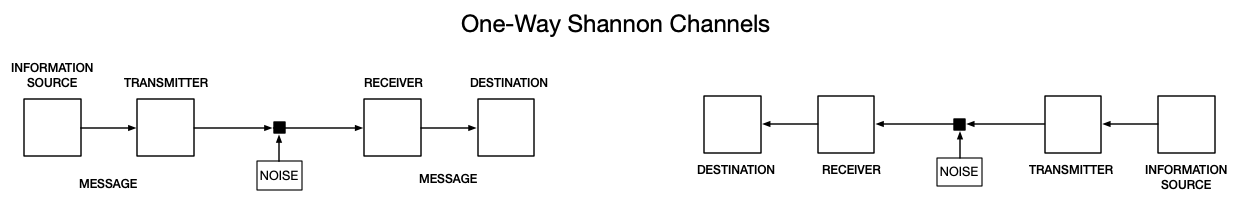
\includegraphics[width=\textwidth]{../figures/One-Way-Shannon.png}
  \caption{Shannon One-Way Channels. }
\end{figure*}

Shannon Channels are normally shown in one \emph{direction} of flow -- from Information source to Information Destination. Here we exploit two-way communication (signaling) Back to Back Channels with immediate (slice by slice) feedback. Then the equations tell us something interesting about the \emph{symmetry} of set reconciliation on both sides of the link.

With back-to-back Shannon Channels, with (immediate) slice by slice feedback, we get Perfect Information Transfer (PIT) \cite{soltted-aloha}. We can therefore dispense with Checksums, CRC's, FEC or even Parity,  because the failure modes these EDC and ECC codes address are already covered by PIT.  This has two advantages:

\begin{itemize}
\item The elimination of spatial redundancy on the wire makes the packets shorter
\item The need to calculate increasingly complex codes reduces computation and energy dissipation on the link
\end{itemize}

\marginnote{Redundancy is a poor crutch when  assumptions about uniform probability distributions are violated (which they almost always are in practice).}

\bigskip \bigskip

\subsection{Metcalfe Half-Duplex}

\begin{figure*}
%  \incplt{acquisition_functions_contours}
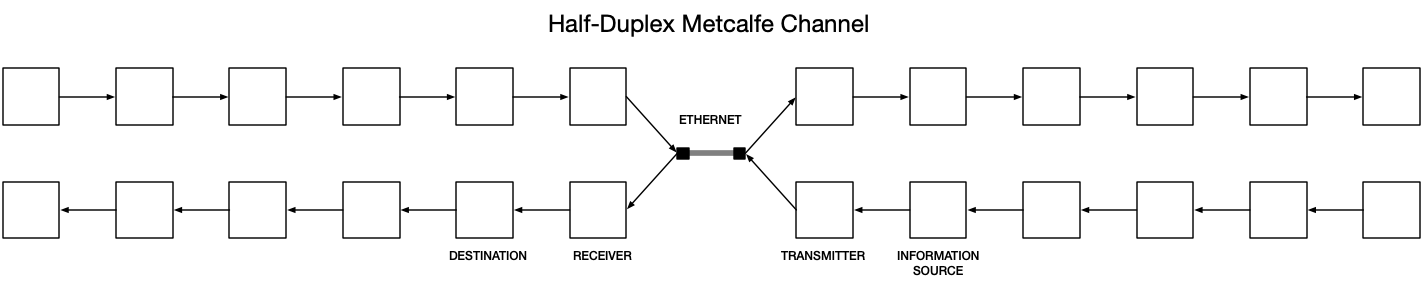
\includegraphics[width=\textwidth]{../figures/Half-Duplex-Metcalfe.png}
  \caption{The original Metcalfe + Boggs Ethernet was a bus. A long cable where `stations' were TAPs on the bus. This meant that each station had to both listen, and transmit from teach tap. In this figure we show two \emph{independent} streams of packets going in opposite direction (forwardpropagation and backpropagation) through a single half-duplex link}
\end{figure*}



\subsection{Metcalfe Half-Duplex Channel}

\begin{figure*}
%  \incplt{acquisition_functions_contours}
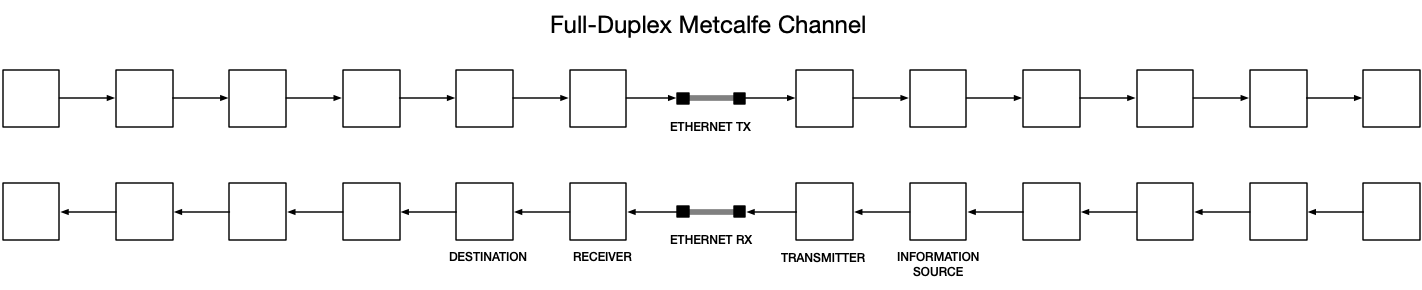
\includegraphics[width=\textwidth]{../figures/Full-Duplex-Metcalfe.png}
  \caption{Modern Ethernet Links are bidirectional; two sub-channels: \\one for transmit,  one for receive}
\end{figure*}



\subsection{Full-Duplex Bi-pipelined Shannon-Metcalfe Channel}

\begin{figure*}
%  \incplt{acquisition_functions_contours}
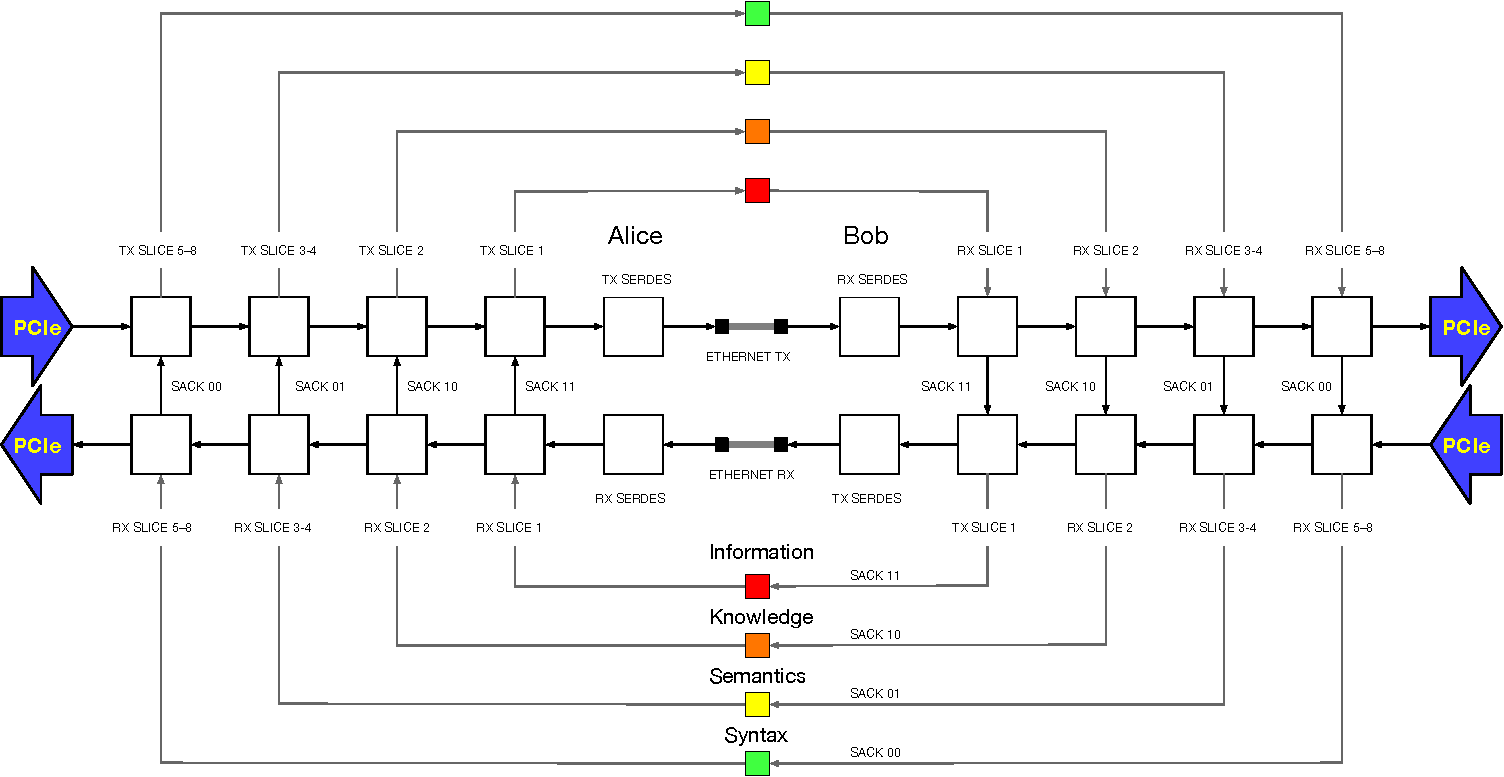
\includegraphics[width=\textwidth]{../figures/Full-Duplex-Bi-Pipelined.pdf}
  \caption{Complete model: Bi-pipelined full duplex exchange of  Æthernet frames. Complete with internal "Slice ACKnowledges" (SACKs) -- sequenced with increasing \emph{common knowledge} depth inside SerDes/FPGA}
\end{figure*}

The figure above is a simple, formally verifiable, mathematical description, from API to bits on the wire (Shannon channel). 

\section{Slice Engine Design}

\subsection{Two independent Metcalfe Channels (Max flow, no Interaction)}

\begin{figure*}
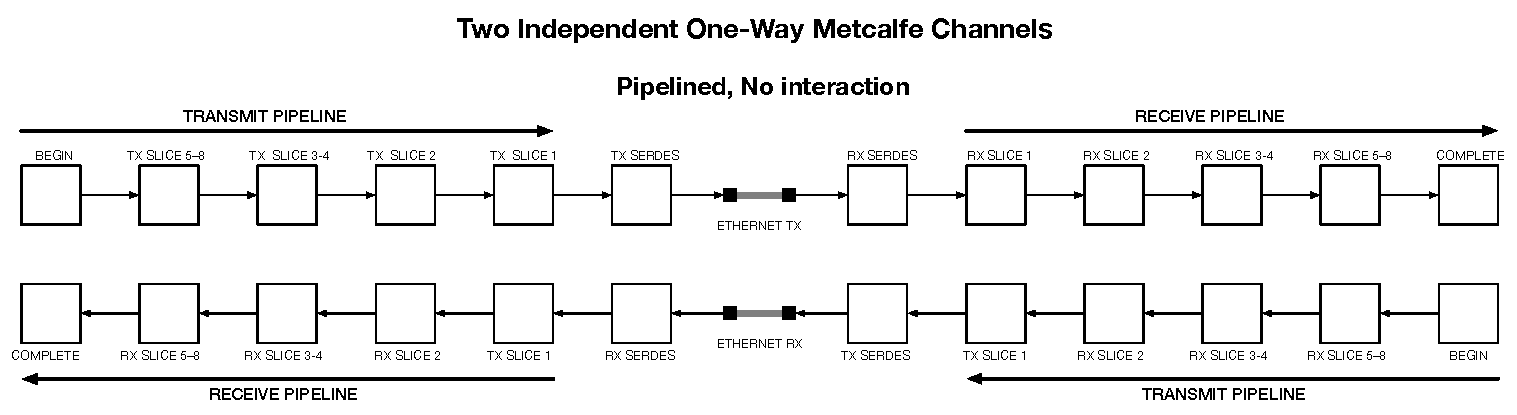
\includegraphics[width=\textwidth]{../figures/Two-Independent-Metcalfe.pdf}
  \caption{Two Independent Metcalfe Channels}
\end{figure*}

\subsection{Internal (SACK) Feedback on last slice}

\begin{figure*}
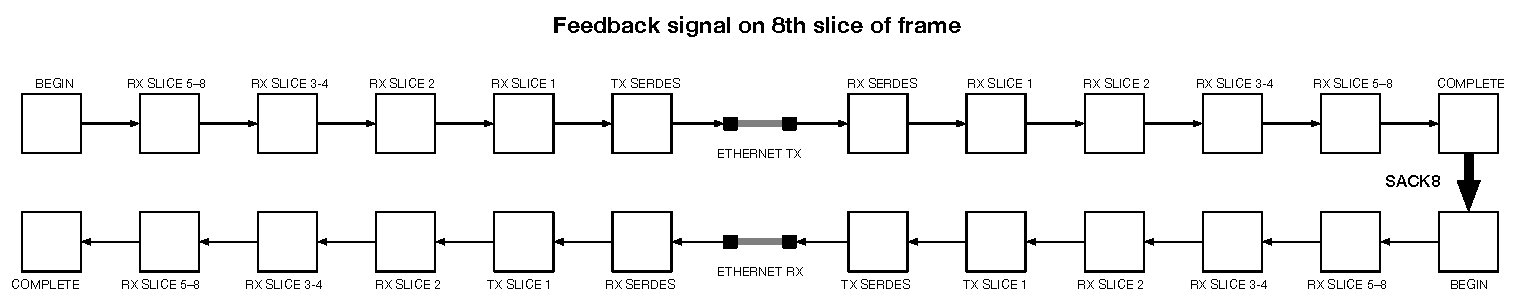
\includegraphics[width=\textwidth]{../figures/feedback-slice-8.pdf}
  \caption{Feedback signal on slice 8}
\end{figure*}

\subsection{Internal (SACK) Feedback on first slice}

\marginnote{See SACK description by Sahas \cite{sahas-02025-1}}

\begin{figure*}
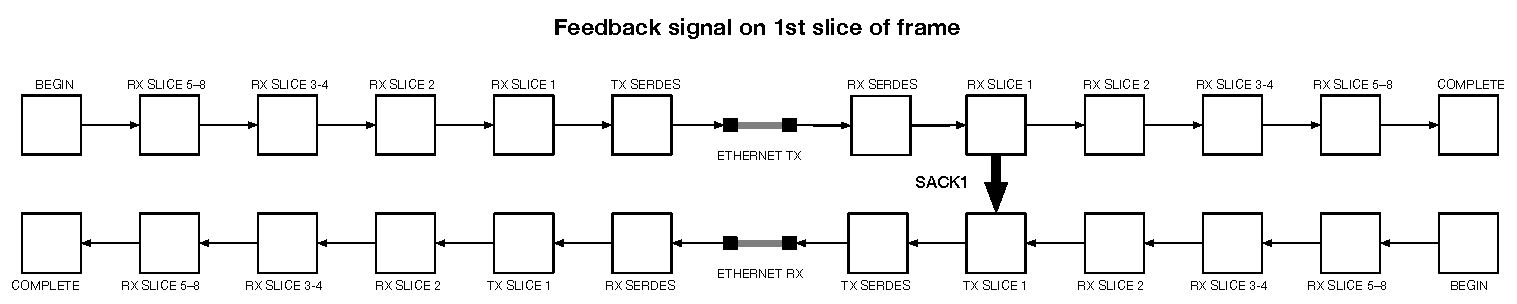
\includegraphics[width=\textwidth]{../figures/Feedback-slice-1.pdf}
  \caption{Feedback signal on slice 1}
\end{figure*}

\newpage
\section{Information, Knowledge, Semantics and Syntax}

%\section*{Distinguishing Information and Knowledge in ML Systems Architecture}
%
%A useful and practical distinction between \textbf{information} and \textbf{knowledge} in machine learning (ML) systems architecture is as follows:
%
%\subsection*{Information}
%Information refers to raw, structured or unstructured data that has been processed enough to be useful, but remains without context or interpretation.
%
%\begin{itemize}
%  \item Typically represented as:
%    \begin{itemize}
%      \item Feature vectors
%      \item Embeddings
%      \item Intermediate model outputs
%      \item Logs, metrics, and labeled datasets
%    \end{itemize}
%  \item Often \textbf{local}, \textbf{transient}, and \textbf{stateless}
%  \item Examples include:
%    \begin{itemize}
%      \item A vector of image pixel values
%      \item An output from a transformer attention head
%      \item A probability distribution over classes
%    \end{itemize}
%\end{itemize}
%
%\subsection*{Knowledge}
%Knowledge refers to contextualized, reusable abstractions derived from information and validated across tasks or environments. It supports generalization and decision-making.
%
%\begin{itemize}
%  \item Typically represented as:
%    \begin{itemize}
%      \item Pretrained model weights
%      \item Learned priors or schemas
%      \item Rules or invariants derived from many examples
%    \end{itemize}
%  \item Often \textbf{global}, \textbf{persistent}, and sometimes \textbf{stateful}
%  \item Examples include:
%    \begin{itemize}
%      \item A pretrained BERT model encoding semantic relationships
%      \item The learned parameters of a convolutional network
%      \item A decision policy in reinforcement learning
%    \end{itemize}
%\end{itemize}
%
%\subsection*{Architectural Distinction}
%
%\begin{table}[h!]
%\centering
%\begin{tabular}{|l|p{5cm}|p{6cm}|}
%\hline
%\textbf{Layer} & \textbf{Role of Information} & \textbf{Role of Knowledge} \\
%\hline
%Input pipeline & Raw data is converted into structured information (e.g., tokens, features) & No knowledge applied yet \\
%\hline
%Model body & Information flows and transforms across layers & Knowledge is encoded in learned weights and internal structure \\
%\hline
%Training loop & Collects and labels information for learning & Updates and refines knowledge via optimization (e.g., backpropagation) \\
%\hline
%Inference system & Uses new input information for prediction & Applies stored knowledge to infer outputs \\
%\hline
%Monitoring \& Feedback & Captures runtime information (e.g., accuracy, drift) & Identifies when stored knowledge needs retraining or fine-tuning \\
%\hline
%\end{tabular}
%\caption{Architectural roles of information and knowledge in ML systems}
%\end{table}
%
%\subsection*{Analogy}
%Information is like \emph{fuel}; knowledge is like the \emph{engine}. The architecture orchestrates the flow of information to refine and apply knowledge efficiently.
%
%
%\title{ALOHA vs Slotted ALOHA}
%%\author{}
%%\date{}
%%
%%\begin{document}
%%\maketitle
%
%%\begin{abstract}
%%This document compares the classical ALOHA protocol with its improved variant, Slotted ALOHA, highlighting differences in their design, collision behavior, and efficiency.
%%\end{abstract}
%
%\section{Introduction}
%
%The \textbf{ALOHA protocol}\sidenote{Developed in the late 1960s at the University of Hawaii for radio communications} allows nodes to transmit packets at any time, leading to frequent collisions. 
%\textbf{Slotted ALOHA}\sidenote{Introduced shortly after by Roberts in 1972}, in contrast, divides time into discrete slots, allowing transmissions only at the beginning of a slot, thereby reducing the chance of collisions.
%
%\section{Comparison Table}
%
%\begin{table}[h]
%\centering
%\begin{tabular}{@{}lll@{}}
%\toprule
%\textbf{Feature} & \textbf{ALOHA} & \textbf{Slotted ALOHA} \\
%\midrule
%Time structure & Any time & Slot-aligned \\
%Collision probability & High & Lower \\
%Efficiency (max) & $\approx 18\%$ (1/2e) & $\approx 37\%$ (1/e) \\
%Implementation complexity & Simple & Needs synchronization \\
%Analogy & Random shouting & Timed shouting \\
%\bottomrule
%\end{tabular}
%\caption{Key differences between ALOHA and Slotted ALOHA.}
%\end{table}
%
% 
%\textbf{ALOHA} allows nodes to transmit without coordination,\sidenote{This freedom results in many partial collisions where packets overlap partially in time.} but suffers from a high collision probability.
%
%\textbf{Slotted ALOHA} improves throughput by enforcing transmission only at predefined time slots,\sidenote{By waiting until the next time slot boundary, nodes avoid partial overlaps.} achieving almost twice the maximum throughput.
%
%Overall, Slotted ALOHA introduces a modest increase in complexity but greatly improves network performance in high-load scenarios.\sidenote{Especially important for early satellite and Ethernet networks.}

%\section{References}
%
%\begin{itemize}
%\item N. Abramson, ``The ALOHA System—Another Alternative for Computer Communications,'' in \textit{Proceedings of the 1970 Fall Joint Computer Conference}, AFIPS Press, 1970.
%\item L. Kleinrock and F. Tobagi, ``Packet Switching in Radio Channels: Part I--Carrier Sense Multiple-Access Modes and Their Throughput,'' \textit{IEEE Transactions on Communications}, vol. 23, no. 12, Dec. 1975.
%\end{itemize}


\section*{Framework: Multiplexed Four Shannon `surprisal' Levels}

In the proposal for subdividing a 64-byte packet into 8-byte slices, we introduce partial acknowledgments (SACKs) at four boundaries (\texttt{11}, \texttt{10}, \texttt{01}, \texttt{00}). Each of these points reveals an \emph{decremented} deeper level of the receiver’s certainty about the data, the hardware, and the appropriate next step in the protocol. We can interpret this progressive certainty in terms of four conceptual \emph{layers} reminiscent of Shannon’s \emph{information} theory, but extended to address knowledge, semantics, and syntax. This layering describes how a receiver (e.g., the SmartNIC) transitions from raw incoming bits to meaningful messages that can be handed off to the host processor.

\subsection*{Layer 1: Information (Surprisal)}

\begin{itemize}
  \item \textbf{Definition:} \emph{Information} at this level is the direct ``yes/no'' answer to a question of interest---the arrival or non-arrival of bits---which Shannon famously treated as the \emph{surprisal} of a received symbol.
  \item \textbf{Context in SACK \texttt{11} (First 8-Byte Slice):}
  \begin{itemize}
    \item When the receiver detects the first 8-byte slice without error, it learns that the link is alive and the data matches expectation (no immediate mismatch).
    \item This is pure \emph{information} because it distinguishes the event ``we \emph{did} receive slice\,\#1 correctly'' from ``we did not.'' 
    \item Mutual information gained: the system confirms a working cable and functional SerDes.
  \end{itemize}
\end{itemize}

\vspace{6pt}

\noindent
At this early stage, we have only answered a \emph{binary} question: ``Did the hardware see valid bits?'' The \emph{surprisal} is that there \emph{were} valid bits, as opposed to no signal or corrupted data.

\subsection*{Layer 2: Knowledge (Captured Information)}

\begin{itemize}
  \item \textbf{Definition:} \emph{Knowledge} arises when the raw bits are \emph{stored} or \emph{captured} in a meaningful structure: for example, as a recognized slice in buffer memory or a pipeline register. 
  \item \textbf{Context in SACK \texttt{10} (Second 8-Byte Slice):}
  \begin{itemize}
    \item By the time the second slice arrives, the receiver has \emph{captured} more bits (16\,bytes so far) and placed them into NIC-internal registers.
    \item It can do further checks: e.g.\ alignment, partial CRC, or expected header fields.
    \item The SACK \texttt{01} confirms that the hardware not only saw valid bits but also placed them in the correct buffer location.
  \end{itemize}
\end{itemize}

\vspace{6pt}

\noindent
Hence, a partial aggregator or parser now \emph{knows} something---the 16\,bytes are indeed recognized and safely stored, awaiting deeper logic to interpret them.

\subsection*{Layer 3: Semantics (Meaning)}

\begin{itemize}
  \item \textbf{Definition:} \emph{Semantics} is where the system decides \emph{what} the bits \emph{mean} in terms of subsequent action: i.e.\ which \emph{state machine} or \emph{processing path} is relevant.
  \item \textbf{Context in SACK \texttt{01} (Slices \#3 and \#4 Arrive):}
  \begin{itemize}
    \item After 32\,bytes are in place, the NIC can do enough partial decoding to see, for instance, which protocol or message type is indicated. 
    \item It can confirm that buffer slots or ring descriptors are available and that the correct state machine is loaded (e.g.\ state machine A for small control frames, or state machine B for streaming payloads).
    \item Once the NIC signals SACK \texttt{10}, the sender learns the hardware has found the data \emph{coherent} enough to continue. The semantics are recognized sufficiently to keep going without hazard.
  \end{itemize}
\end{itemize}

\vspace{6pt}

\noindent
Thus, the receiver has passed from raw knowledge of the bits (Levels 1--2) to \emph{semantic} interpretation (Level\,3) that tells it \emph{how} to proceed and \emph{which} internal resources or state machines to activate.

\subsection*{Layer 4: Understanding (Syntax)}

\begin{itemize}
  \item \textbf{Definition:} \emph{Understanding} here refers to recognizing that the message fits into a finite set of \emph{concepts or message types} accepted by the NIC---in other words, a correct \emph{syntax} recognized by the hardware. 
  \item \textbf{Context in SACK \texttt{00} (Slices \#5--\#8 Arrive):}
  \begin{itemize}
    \item This final partial-ACK boundary shows that the full 64\,bytes match a legitimate frame or message layout. 
    \item The NIC is ready to push the message onto the PCIe bus or onto an internal ring buffer for the Host processor. 
    \item It implies the NIC has full \emph{understanding} of how to finalize the packet, classify it, and pass it upstream for higher-level processing.
  \end{itemize}
\end{itemize}

\vspace{6pt}

\noindent
In short, at this stage, the hardware knows that it has recognized \emph{which} valid format or syntax the message belongs to and that no further layer-2 repairs are needed.

\section*{Why the Four Layers Matter}

\begin{enumerate}
\item \textbf{Information (Surprisal)} ensures the physical channel is alive and bits can be reliably seen.
\item \textbf{Knowledge (Captured Information)} confirms the bits are stored in correct buffers or registers---no accidental misalignment.
\item \textbf{Semantics (Meaning)} ensures the logic knows \emph{how} to handle the data and which internal processes to activate.
\item \textbf{Understanding (Syntax)} verifies the packet’s higher-level consistency and classifies it for final delivery to the host.

\end{enumerate}

Each SACK boundary (\texttt{11}, \texttt{10}, \texttt{01}, \texttt{00}) maps neatly onto these four conceptual levels. As soon as the sender receives each partial ACK, it gains confidence that the receiver has \emph{progressed} one step deeper in turning raw signals (bits) into a \emph{fully understood} data frame and state machine context. This four-layer design captures a more Shannon-like architecture in which each additional SACK message not only signals success \emph{so far}, but also narrows the set of potential failure modes and clarifies how the data \emph{will} be handled.



\section{Shannon Slots (2nd half of document)}

\subsection{Single + Dual Channel}
\begin{marginfigure}
  \centering
  \includegraphics[width=1.2\linewidth]{../figures/One-Way-Shannon-LR.pdf}
%  \caption{One Way Shannon Channel \emph{Left to Right causality}}

\end{marginfigure}

\begin{marginfigure}t
  \centering
  \includegraphics[width=1.2\linewidth]{../figures/One-Way-Shannon-RL.pdf}
%  \caption{One Way Shannon Channel \emph{Right to Left causality}}
\vspace{10pt}
\end{marginfigure}



\begin{itemize}
\item A single Channel Shannon Channel is the conventional view of Information
\marginnote{Key aspects of Shannon Channels  are already “reversible” based on \emph{mutual} and \emph{consistent} information; these are symmetric in time in our model for Common Knowledge.   [See JV Stone: \href{https://arxiv.org/pdf/1802.05968}{Information Theory: A Tutorial Introduction}] }
%\marginnote{Recommended Reading: \href{https://arxiv.org/pdf/1802.05968}{Information Theory: A Tutorial Introduction}}

\item The former is statistical (correlated only), the latter is 100\% consistent.
\item Our Reversible Dual Channel Shannon model enables both full reversibility and provides new opportunities for Error detection and Correction
\item The theory is fully consistent with the scientific literature, but applying it to short cables provides a new opportunity - within racks, and chiplet meshes
\item This presentation is patentable new IP. The AEIA plans to make any IP necessary for the implementation of Open Atomic Ethernet, available with a free license to compliant products (those that pass the conformance and compatibility tests, and any trademarks, through the IEEE if they choose to accept this as a formal standards track.
\item It applies specifically to the “Sahas information model (see slides at end)
\item This is the foundation for a new model for a Product: Link Failure Detector 
\end{itemize}

%\begin{marginfigure}
%\href{https://x.com/colmmacc/status/1146429508993503234?s=61}{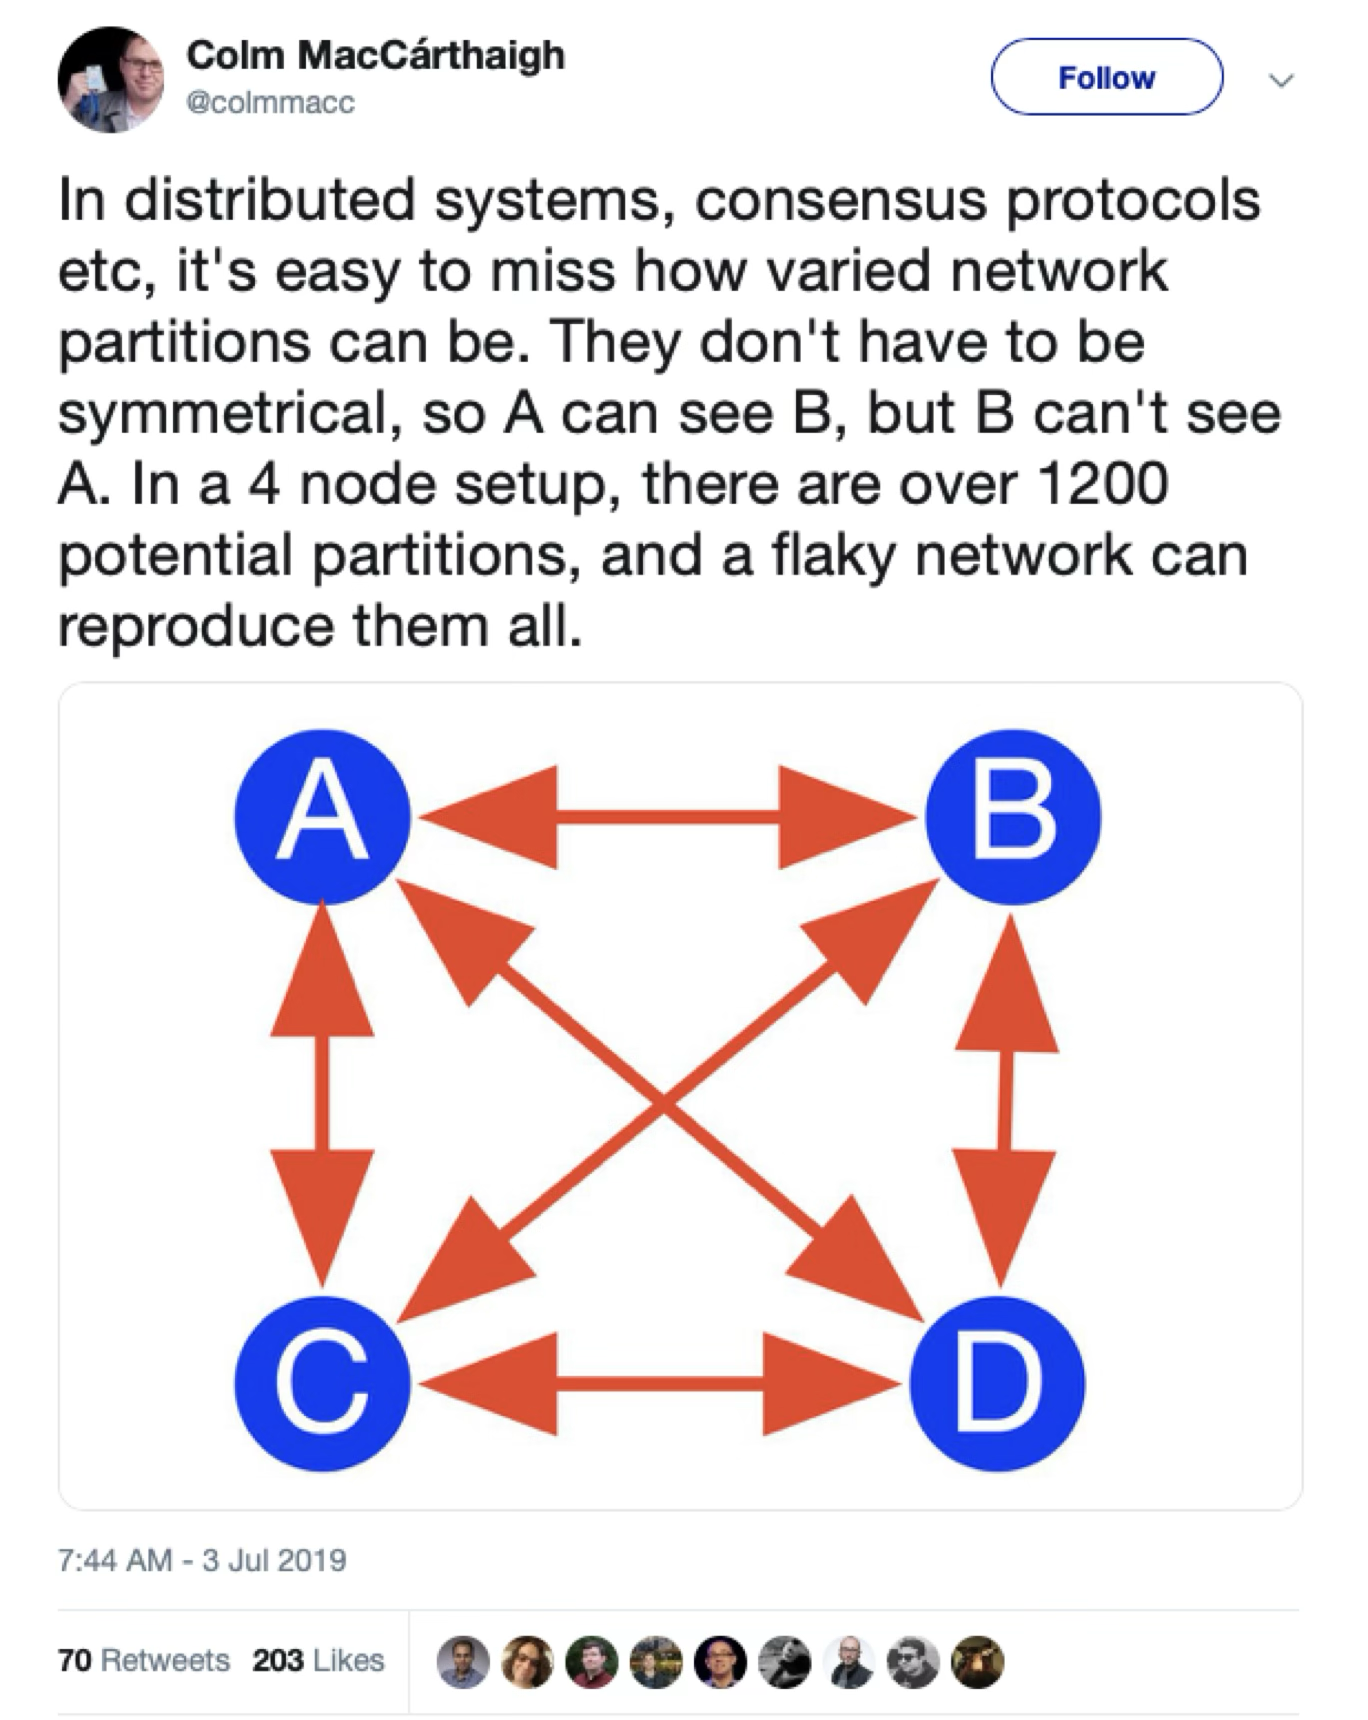
\includegraphics[width=\linewidth]{../Figures/Flakey-Network.png}}
%%  \caption{\href{https://x.com/colmmacc/status/1146429508993503234?s=61}{X/Twitter}}
%\end{marginfigure}


\section{Shannon Reversibility Levels}

\begin{itemize}
\item Information Slots (surprisal)
\item Knowledge Slots (captured information)
\item Semantic Slots (meaning)
\end{itemize}

\subsection{Slot Reconciliation Protocol}

[Reference Pat's favorite paper, and wiki session he gave + Transcript

\begin{fullwidth}
\begin{figure}[ht]
  \centering
  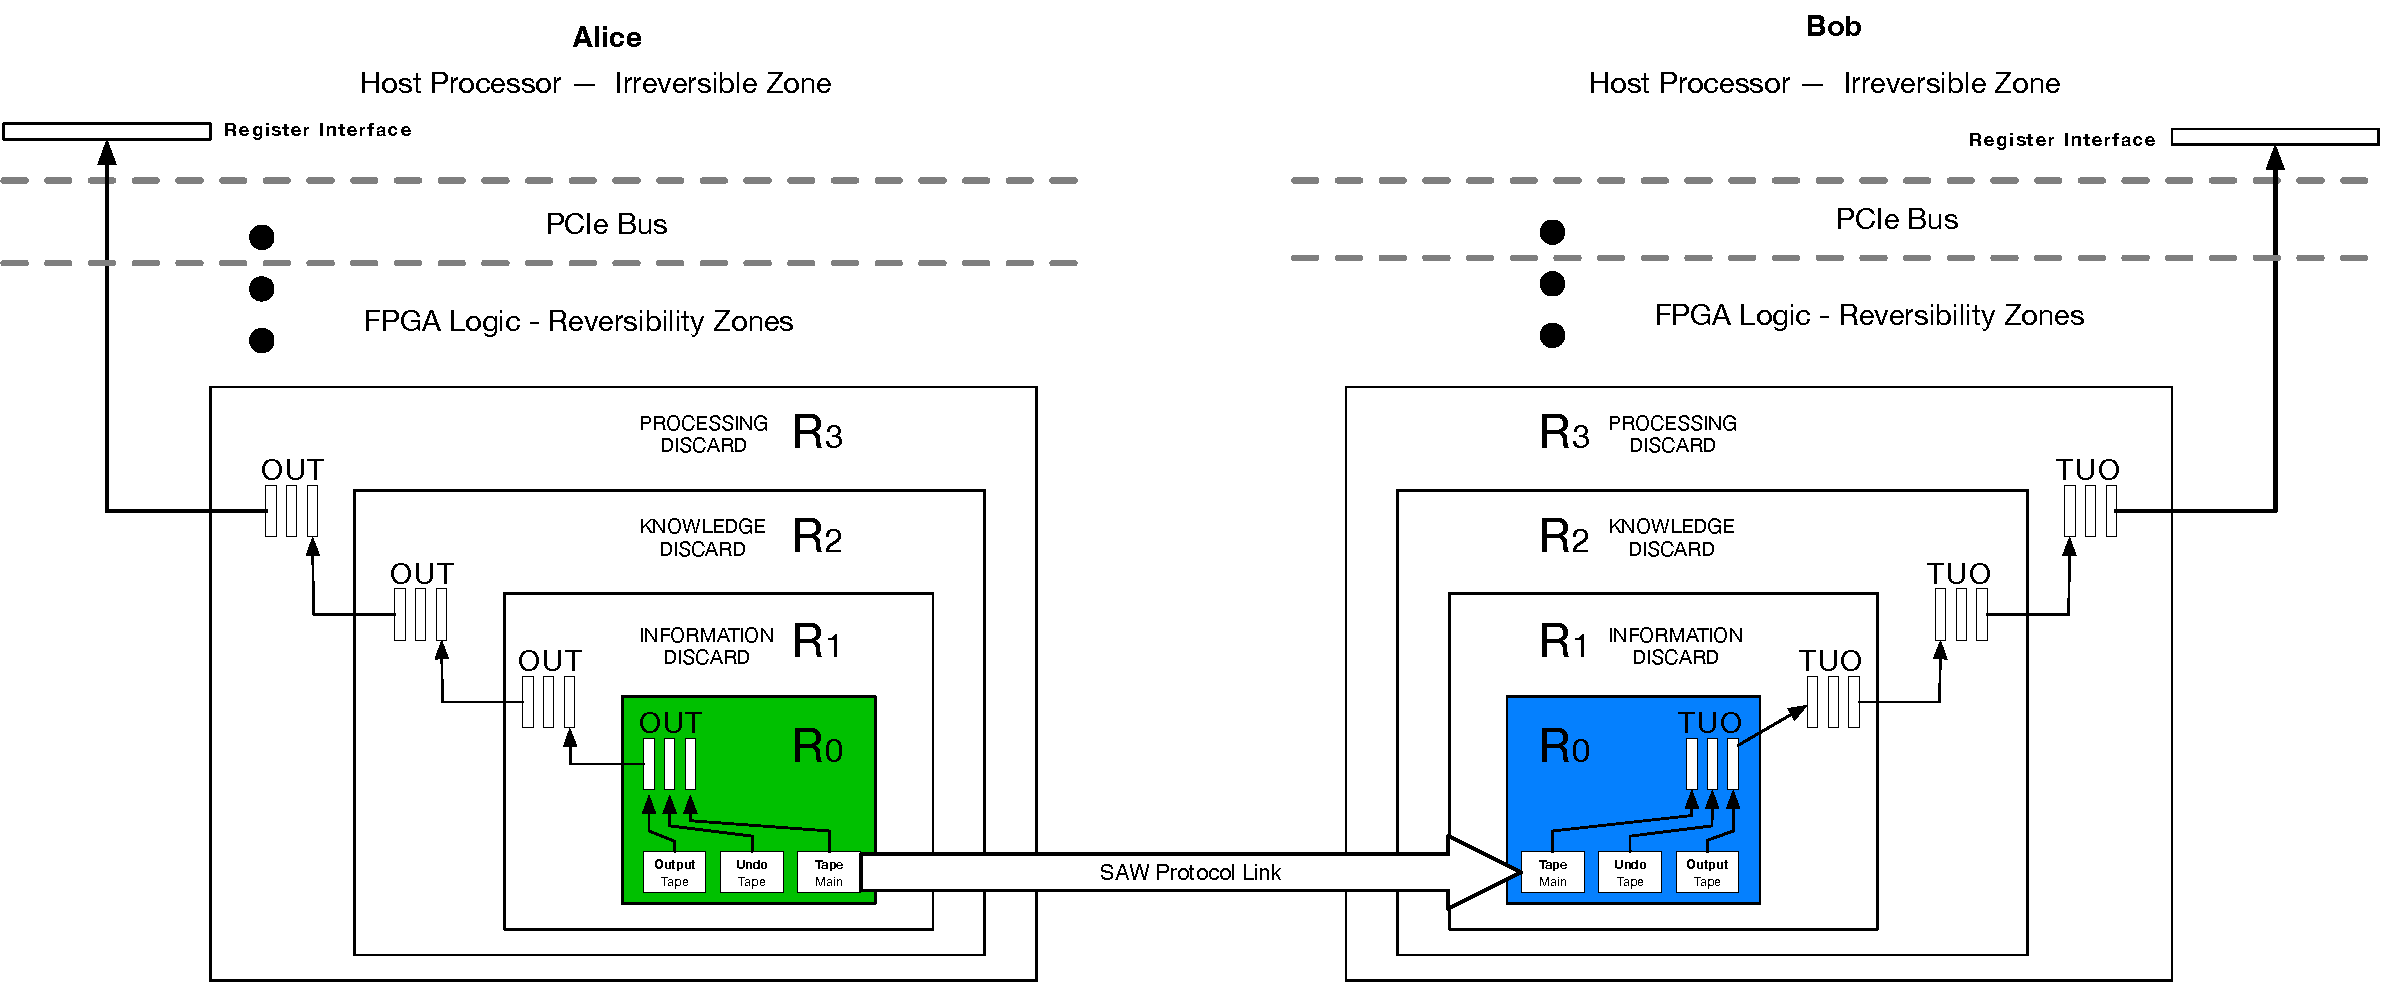
\includegraphics[width=1.5\linewidth]{../figures/Shannon-Reversibility-Levels.pdf}

\end{figure}
\end{fullwidth}


\clearpage
\section{When Two Shannon Channels are connected Back to Back}

\begin{figure}[ht]
  \caption{Shannon Slots.}
  \centering
  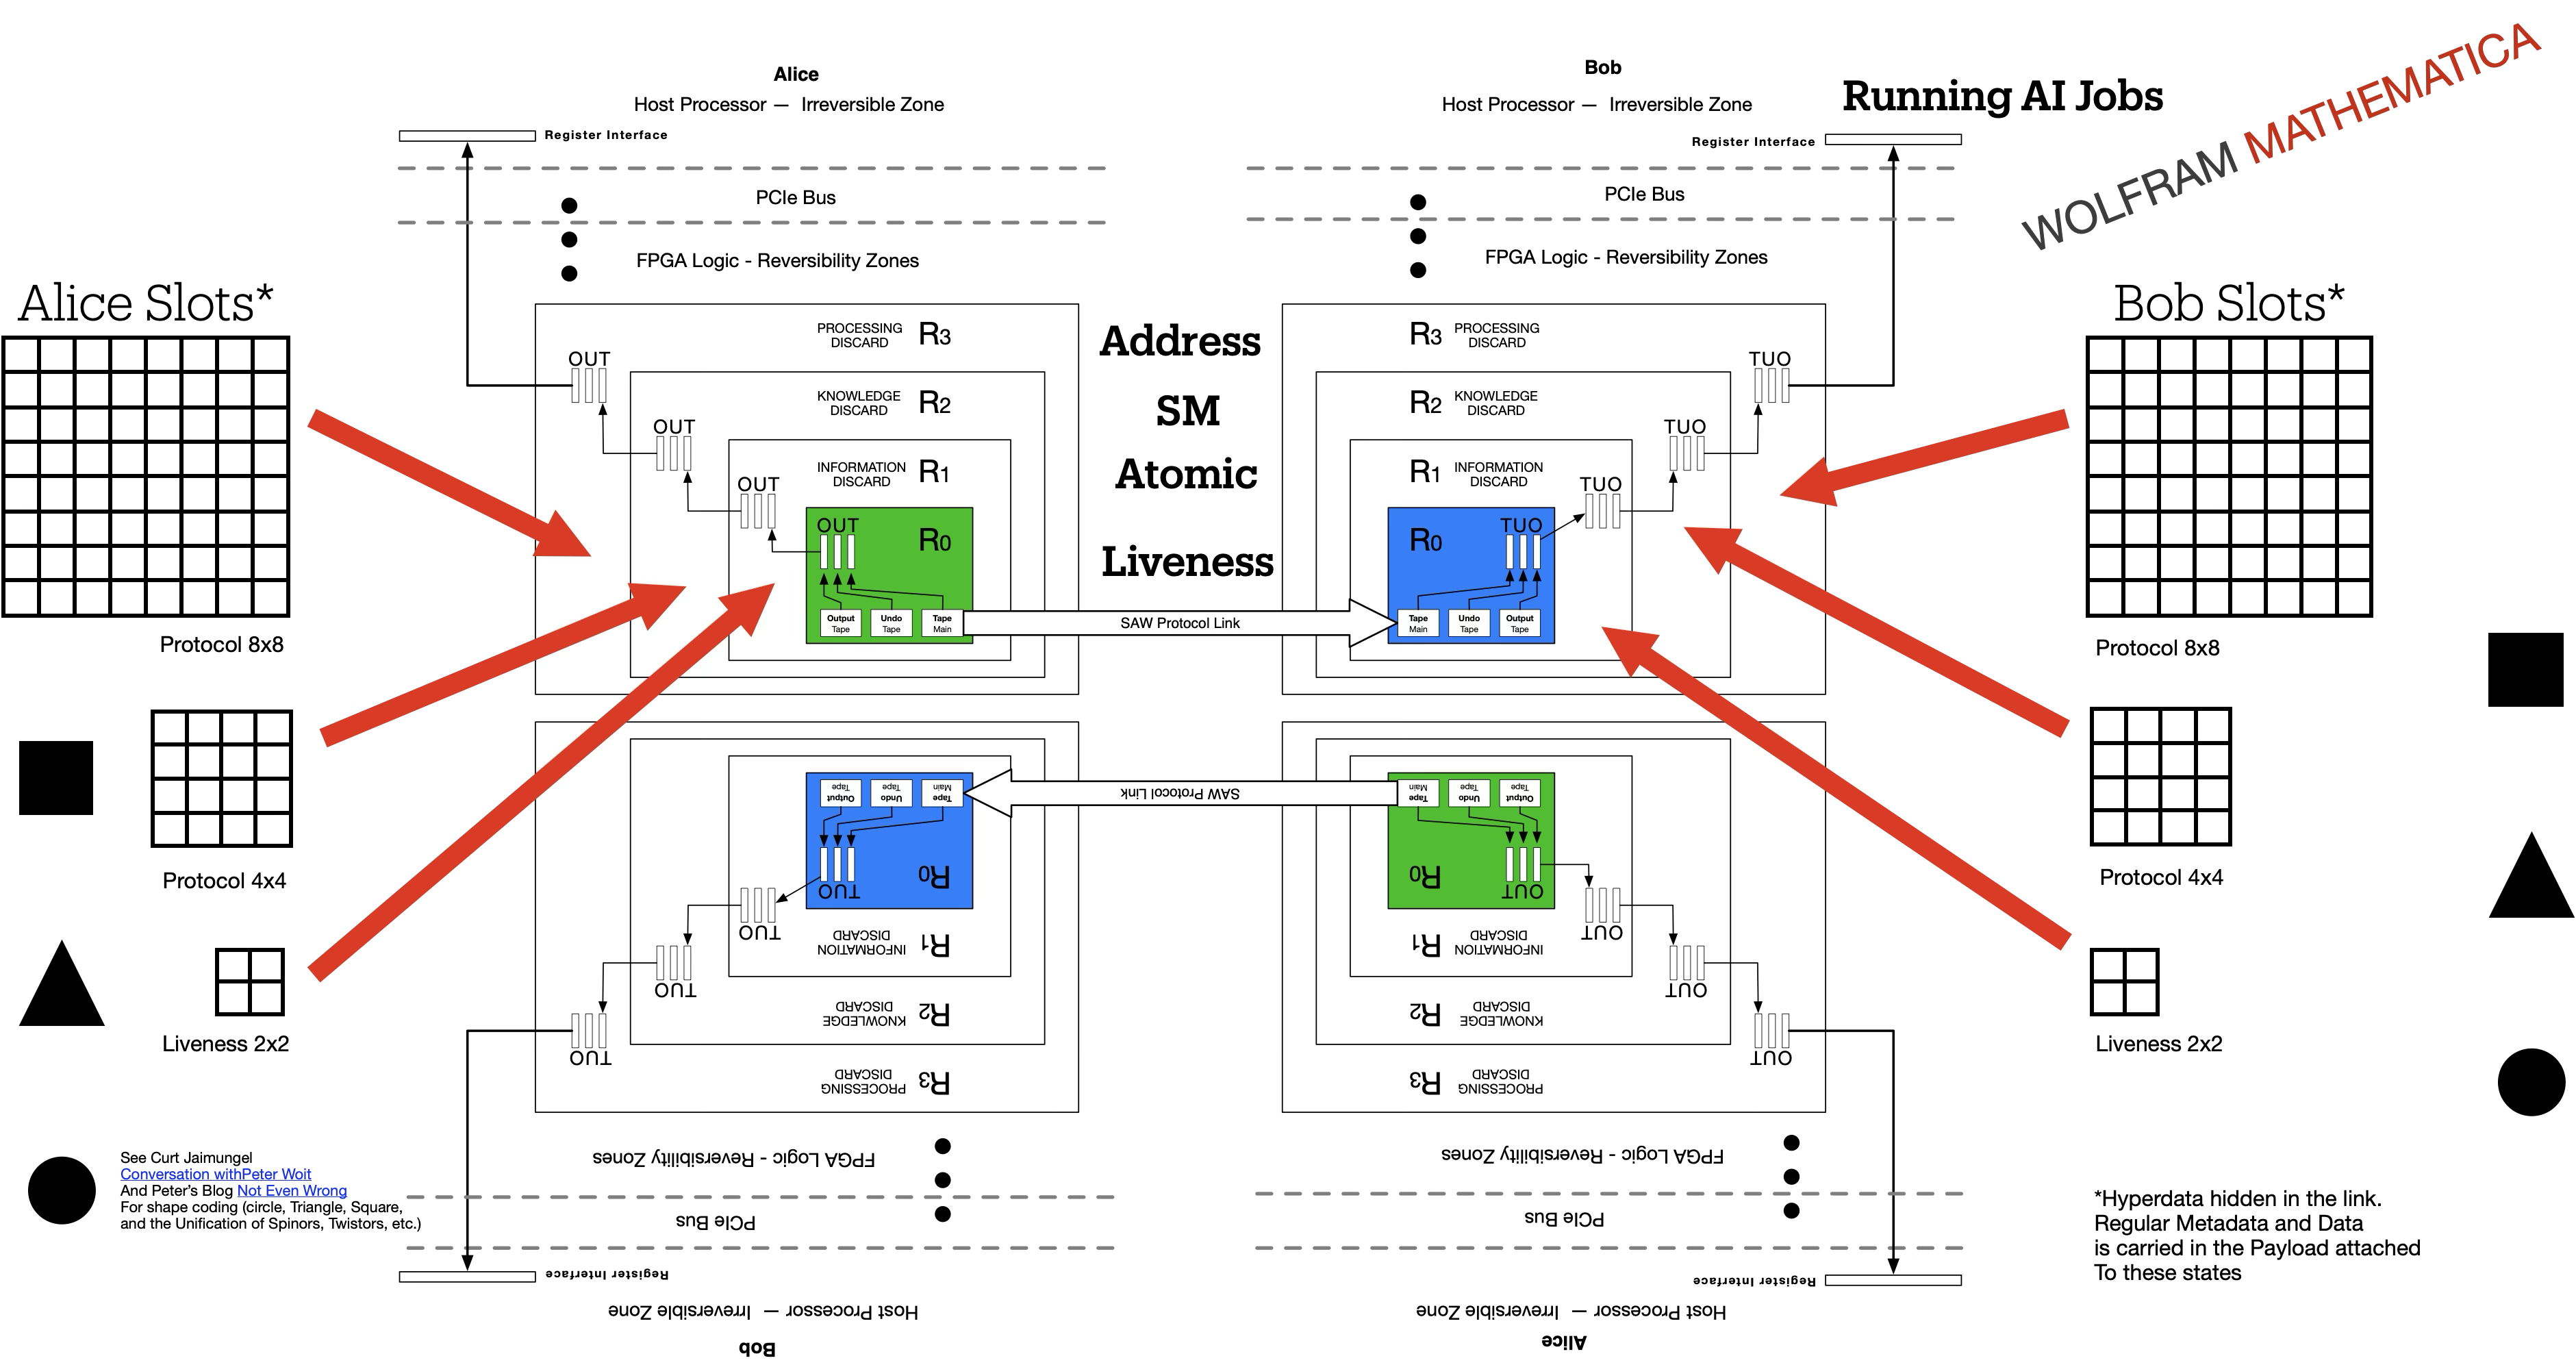
\includegraphics[width=1.6\linewidth]{../figures/Shannon-slots.png}
  \caption{Shannon Slots.}
\end{figure}


%COPIED FROM Acknowledgements in Space Time


\section*{Architectural Framework: Four Shannon-like Levels}

In the proposal for subdividing a 64-byte packet into 8-byte slices, we introduce partial acknowledgments (SACKs) at four (decrementing) boundaries (\texttt{11}, \texttt{10}, \texttt{01}, \texttt{00}). Each of these points reveals an incrementally deeper level of the receiver’s certainty about the data, the hardware, and the appropriate next step in the protocol. We can interpret this progressive certainty in terms of four conceptual \emph{layers} reminiscent of Shannon’s \emph{information} theory, but extended to address knowledge, semantics, and understanding. This layering describes how a receiver (e.g., the SmartNIC) transitions from raw incoming bits to meaningful messages that can be handed off to the host processor.

\marginnote{Back-to-Back (B2B) Shannon Channels are “Perfect Information Feedback” (PIF) as senders see their own transmitted packet returning back from the receiver and thus can detect channel errors.  Thus making CRCs Checksums, Parity and FEC unnecessary.
Similar to "Perfect Information Feedback" in: \href{https://dl.acm.org/doi/pdf/10.1145/1499586.1499751}{Norm Abramson, “Packet switching with satellites,” NCC, 1973}}

\subsection*{Layer 1: Information (Surprisal)}

At the first level, information refers to the direct "yes/no" answer to a question of interest: the arrival or non-arrival of bits, which Shannon famously treated as the surprisal of a received symbol. At the SACK \texttt{00} boundary, when the receiver detects the first 8-byte slice without error, it learns that the link is alive and that the data matches expectations (i.e., no immediate mismatch). This is pure information because it distinguishes the event "we did receive slice \#1 correctly" from "we did not." The mutual information gained here confirms a working cable and a functional SerDes.

At this early stage, the question posed is binary: "Did the hardware see valid bits?" The surprisal is that valid bits were received, as opposed to no signal or corrupted data.

\subsection*{Layer 2: Knowledge (Captured Information)}

The second layer, knowledge, arises when the raw bits are stored or captured in a meaningful structure. This could be as simple as a recognized slice stored in buffer memory or a pipeline register. By the time the second slice arrives, the receiver has captured more bits—16 bytes in total—and placed them into NIC-internal registers. It can then perform further checks, such as alignment, partial CRC, or checking for expected header fields. The SACK \texttt{01} confirms that the hardware not only saw valid bits but also placed them in the correct buffer location.

At this point, the system has a partial understanding of the data. It knows that the 16 bytes are recognized and safely stored, awaiting deeper logic to interpret them.

\subsection*{Layer 3: Semantics (Meaning)}

The third layer, semantics, involves the system deciding what the bits mean in terms of subsequent action. This layer determines which state machine or processing path is relevant for the given data. At the SACK \texttt{10} boundary, after 32 bytes have been received, the NIC has gathered enough information to partially decode the data. For example, it might be able to determine which protocol or message type is indicated. The NIC can confirm that buffer slots or ring descriptors are available and that the correct state machine is loaded (e.g., state machine A for small control frames, or state machine B for streaming payloads).

Once the NIC signals SACK \texttt{10}, the sender learns that the hardware has found the data coherent enough to continue. The semantics are recognized sufficiently to proceed without hazard. The receiver has now moved from simply knowing the bits are correct (Layers 1 and 2) to understanding how to proceed and which internal resources or state machines to activate.

\subsection*{Layer 4: Understanding (Syntax)}

The final layer, understanding, refers to the recognition that the message fits into a finite set of concepts or message types that the NIC accepts. This implies that the message has a correct syntax recognized by the hardware. At the SACK \texttt{11} boundary, which occurs when slices 5–8 arrive, the full 64 bytes have been received and match a legitimate frame or message layout. The NIC is now ready to push the message onto the PCIe bus or an internal ring buffer for the host processor.

At this stage, the NIC has a full understanding of the message, knowing exactly how to finalize the packet, classify it, and pass it upstream for higher-level processing. No further layer-2 repairs are needed, and the message is ready for the next step in the protocol.



%
%\section*{Why the Four Layers Matter}
%
%\begin{enumerate}
%\item \textbf{Information (Surprisal)} ensures the physical channel is alive and bits can be reliably observed by the receiving SerDes.
%\item \textbf{Knowledge (Captured Information)} confirms the bits are captured correctly in registers or buffers ---no accidental misalignment.
%\item \textbf{Semantics (Meaning)} ensures the logic knows \emph{how} to synchronize the appropriate state machines in their forward (or backward) direction.
%\item \textbf{Understanding (Syntax)} verifies the packet’s higher-level consistency and classifies it for final delivery to the host.
%
%\end{enumerate}
%
%Each SACK boundary (\texttt{00}, \texttt{01}, \texttt{10}, \texttt{11}) maps neatly onto these four conceptual leaps. As soon as the sender receives each partial ACK, it gains confidence that the receiver has \emph{progressed} one step deeper in turning raw signals (bits) into a \emph{fully understood} data frame. This four-layer design captures a more Shannon-like architecture in which each additional SACK message not only signals success \emph{so far}, but also narrows the set of potential failure modes and clarifies how the data \emph{will} be handled.



\clearpage
\begin{fullwidth}
\begin{figure}[ht]
  \centering
 %   \caption{\vspace{-10pt}Shannon Slots.}
  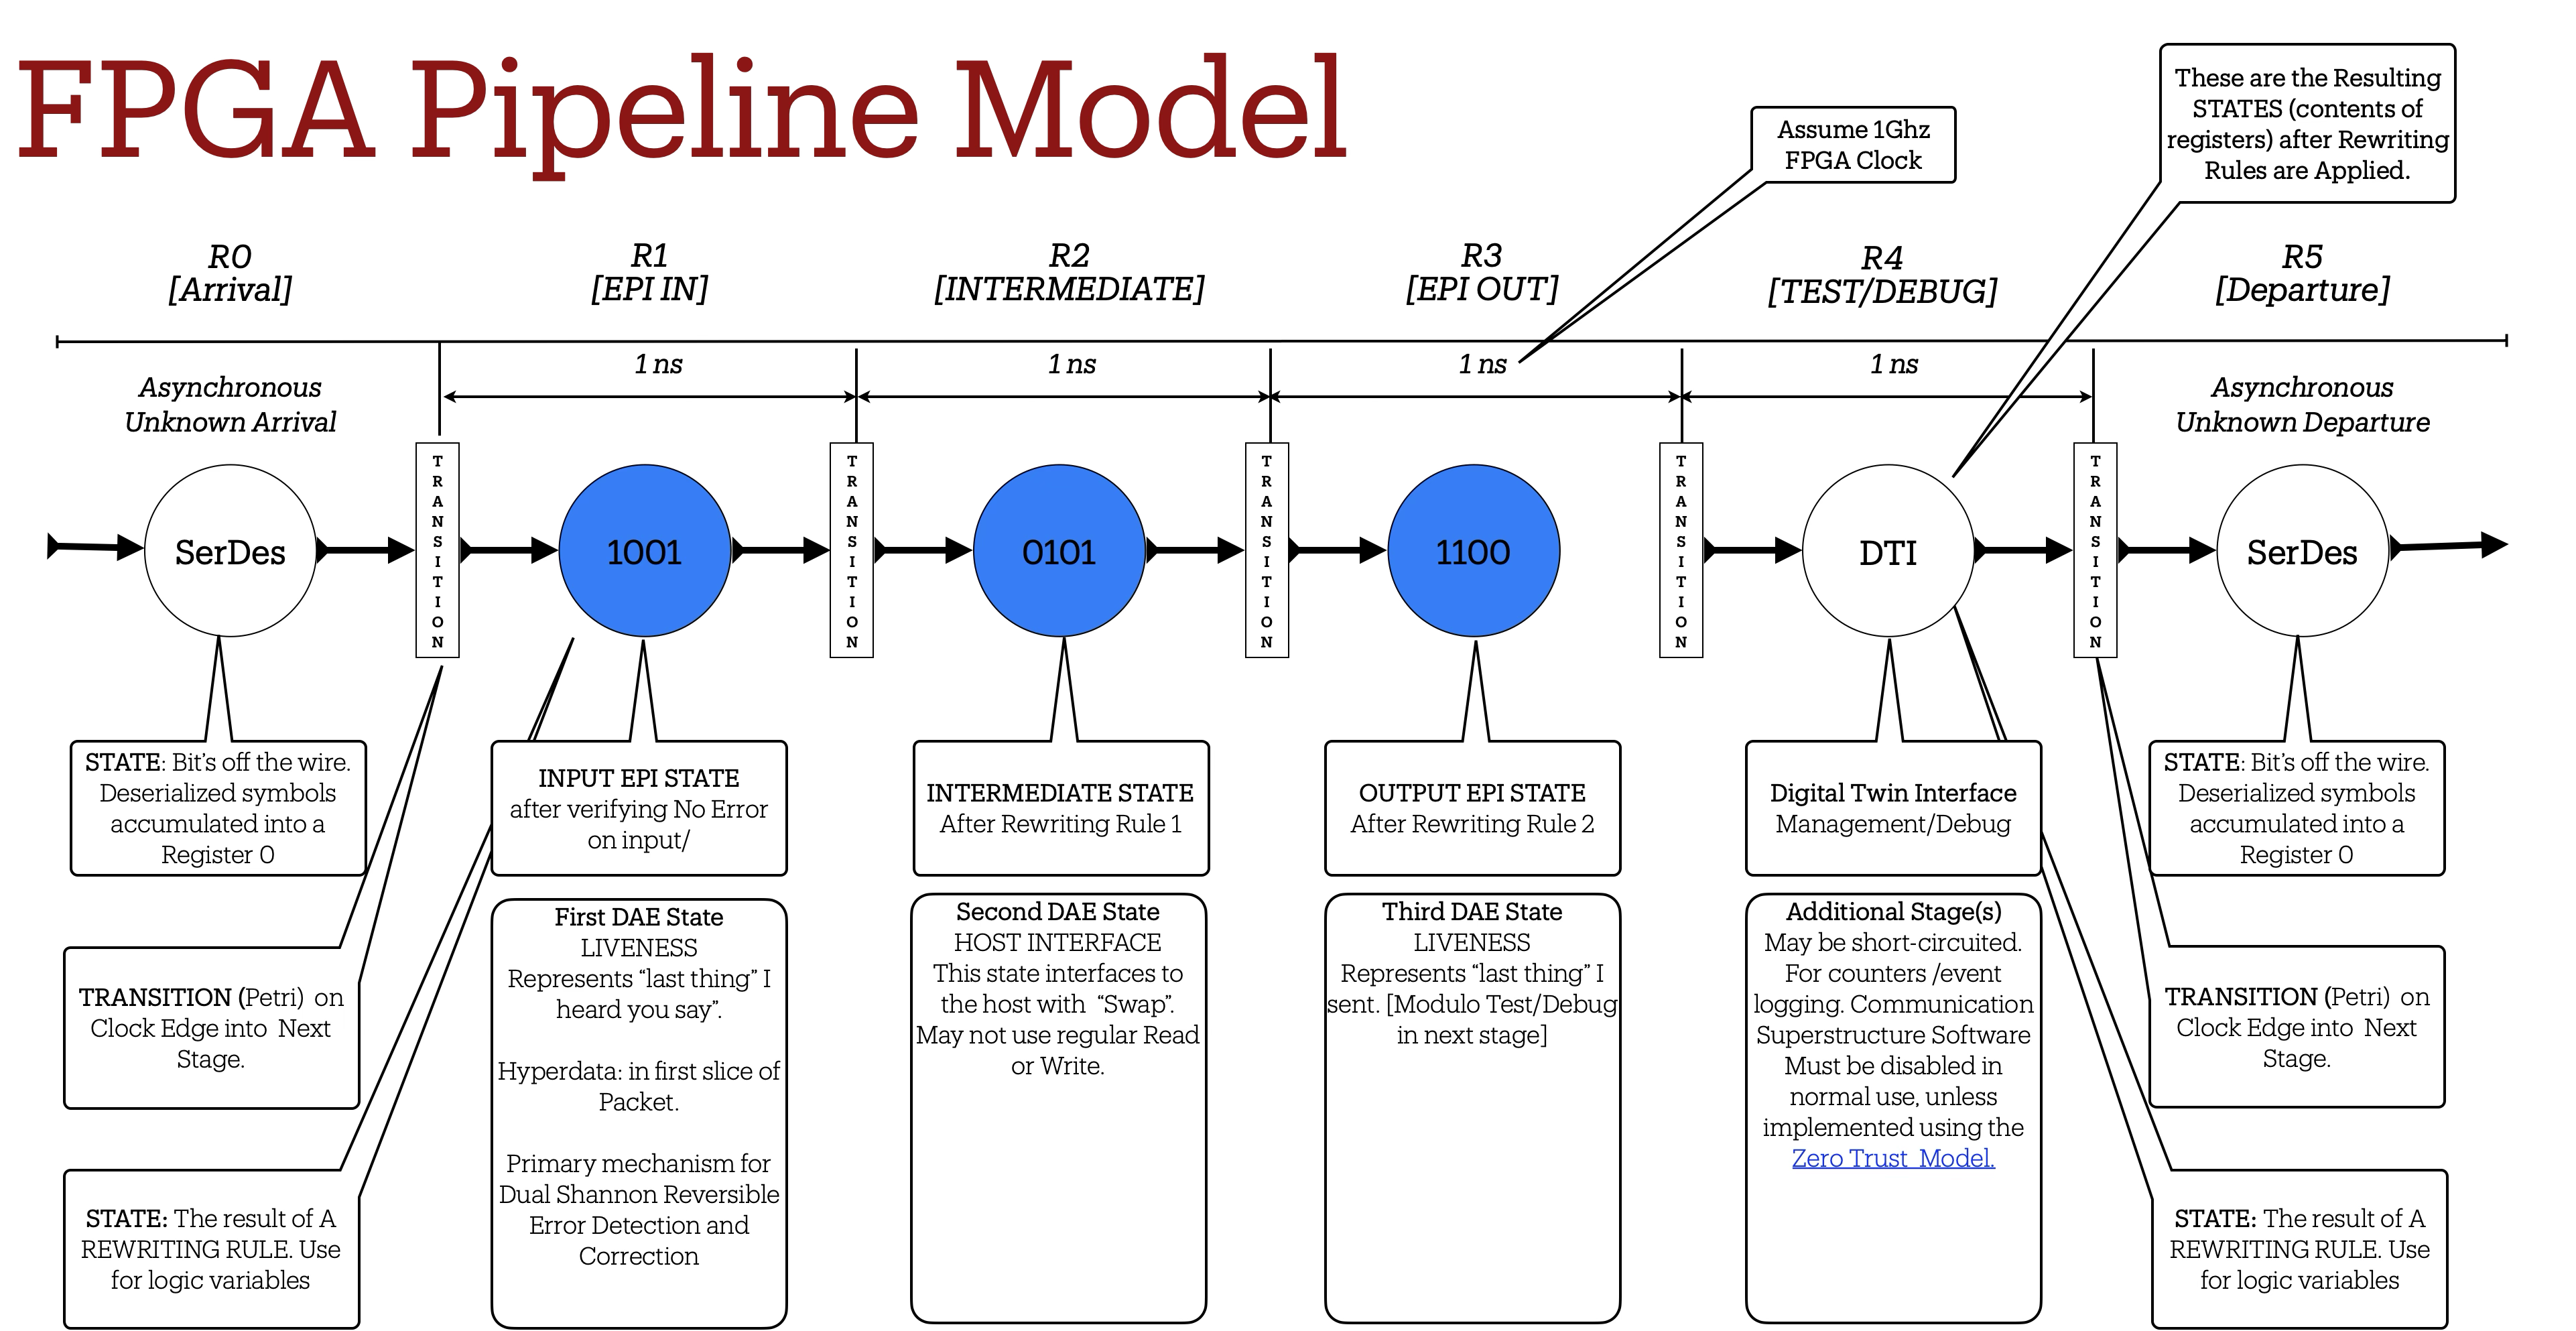
\includegraphics[width=1.5\linewidth]{../figures/FPGA-Pipeline-Model.png}

\end{figure}
\end{fullwidth}
  
\section{FPGA Pipeline Model}


\end{document}

 
